\documentclass[conference]{IEEEtran}
\IEEEoverridecommandlockouts
% The preceding line is only needed to identify funding in the first footnote. If that is unneeded, please comment it out.
\usepackage{cite}
\usepackage{amsmath,amssymb,amsfonts}
\usepackage{algpseudocode}
\usepackage{algorithm}
\usepackage{graphicx}
\usepackage{textcomp}
\usepackage{xcolor}
\usepackage{nicefrac}
\usepackage[frozencache,cachedir=.]{minted}
\usepackage{pgfplots}
\usepackage[english]{babel}
\usepackage{amsthm}
\usepackage{booktabs}

\newtheorem{theorem}{Theorem}
\newtheorem{corollary}{Corollary}[theorem]
\newtheorem{lemma}[theorem]{Lemma}

\newcommand{\floor}[1]{\lfloor #1 \rfloor}
\newcommand{\ceil}[1]{\lceil #1 \rceil}

\graphicspath{{./figures/}}

\def\BibTeX{{\rm B\kern-.05em{\sc i\kern-.025em b}\kern-.08em
    T\kern-.1667em\lower.7ex\hbox{E}\kern-.125emX}}
\begin{document}

%\title{Accelerate Off-policy Reinforcement Learning on Multicore Shared Memory System*\\
% {\footnotesize \textsuperscript{*}Note: Sub-titles are not captured in Xplore and
% should not be used}
%\thanks{This work is supported by xxx under award xxx.}
%}

\title{Parallel Actors and Learners: A Framework for Generating Scalable RL Implementations*\\
% {\footnotesize \textsuperscript{*}Note: Sub-titles are not captured in Xplore and
% should not be used}
\thanks{This work has been sponsored by the U.S. Army Research Office (ARO) under award number W911NF1910362 and the U.S. National Science Foundation (NSF) under award numbers 2009057.}
}

\author{\IEEEauthorblockN{Chi Zhang}
\IEEEauthorblockA{\textit{Department of Computer Science} \\
\textit{University of Southern California}\\
Los Angeles, USA \\
zhan527@usc.edu}
\and
\IEEEauthorblockN{Sanmukh Rao Kuppannagari, Viktor K Prasanna}
\IEEEauthorblockA{\textit{Department of Electrical and Computer Engineering} \\
\textit{University of Southern California}\\
Los Angeles, USA \\
kuppanna@usc.edu, prasanna@usc.edu}
}

\maketitle

%auto-ignore
We introduce a new language representation model called {\bf \bert}, which stands for \textbf{B}idirectional \textbf{E}ncoder \textbf{R}epresentations from \textbf{T}ransformers. Unlike recent language representation models~\cite{peters-etal:2018:_deep, radford-etal:2018},  \bert is designed to pre-train deep bidirectional representations from unlabeled text by jointly conditioning on both left and right context in all layers. As a result, the pre-trained BERT model can be fine-tuned with just one additional output layer to create state-of-the-art models for a wide range of tasks, such as question answering and language inference, without substantial task-specific architecture modifications. 

\bert is conceptually simple and empirically powerful. It obtains new state-of-the-art results on eleven natural language processing tasks, including pushing the GLUE score to 80.5\% (7.7\% point absolute improvement), MultiNLI accuracy to 86.7\% (4.6\% absolute improvement), SQuAD v1.1 question answering Test F1 to 93.2 (1.5 point absolute improvement) and SQuAD v2.0 Test F1 to 83.1 (5.1 point absolute improvement).



\begin{IEEEkeywords}
parallel reinforcement learning, prioritized replay buffer, parameter server
\end{IEEEkeywords}

\section{Introduction}\label{sec:introduction}

From immersive communications, games, virtual production, to virtual try-on and virtual fitting rooms, having an accurate 3D presentation of the body of a person is fundamental. For this, one would typically need to use a professional 3D capture stage with many cameras pointing at the person in the center of the stage, and then put all the videos together using a 3D reconstruction algorithm, such as the ones proposed by \cite{guo2019relightables}, \cite{collet2015high} or \cite{pages2018affordable}. These setups are complex (huge amount of data to manage, complicated calibration processes, high processing times) and expensive (a high number of cameras, professional lighting, computers, GPUs, networks and more), so to overcome these challenges, modern deep learning techniques aim to simplify the capture process by replacing the multi-camera setup with a single camera, from a single viewpoint. For example, \cite{saito2019pifu}, \cite{saito2020pifuhd}, and \cite{xiu2022icon} generate a full body 3D model of a person, \cite{escribano2022texture} propose a way to generate the textures of occluded areas. However, all these techniques output relatively low-resolution considering the target application, and they struggle with complicated poses where depth is difficult to convey from a single viewpoint.

To overcome these challenges, some approaches include additional information into the capturing process, including depth, which typically comes from a consumer-level depth sensor. Although new generation consumer-level depth sensors have significantly improved during the last few years, they still present high levels of noise and sometimes fail to capture details when the subjects are at a distance where their body can be fully captured (at around 2m and farther), and they are still sensitive to sun light (which interferes with the infra-red light these sensors typically use), dark materials (which absorb infra-red light) and non-Lambertian surfaces. 

In this work, we propose a new approach to generate high-resolution depth maps of humans using a single low-resolution image as input, using denoising diffusion probabilistic models (DDPMs). Our multi-modal DDPM was trained using high-resolution depth maps, extracted from a large dataset of photorealistic 3D models captured by Volograms \citep{volograms2021}, which allows us to obtain depth maps with higher accuracy than consumer-level depth sensors.

% Featured Image
\begin{figure}[t]
  \centering
  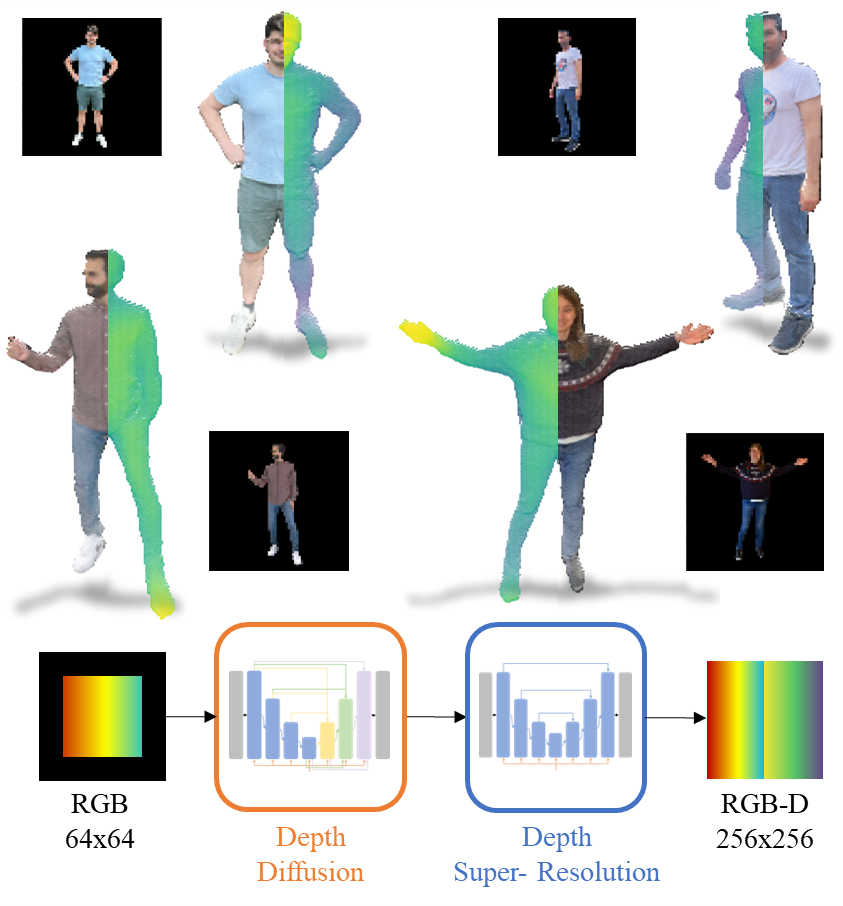
\includegraphics[width=0.99\linewidth]{illustrations/featured_image.png}
  \caption{Our \modelname{} framework generates a high-resolution RGB-D image from a low-resolution RGB image of humanoid subjects. First, a low resolution depth map is generated using a conditional DDPM. Then, the depth is upsampled to a higher resolution using a second DDPM.}
  \label{fig:featured_image}
\end{figure}

Following the taxonomy for multi-modal deep learning systems by \cite{zhan_multimodal_2022} we frame \modelname{} as a multi-modal generative translation task using a joint data representation of our input modalities RGB and depth. No alignment is performed between these modalities since our data is perfectly aligned during generation. We further perform parallel data co-learning since our RGB and depth pairs inherently share a direct correspondence between their instances.

We summarize our main contributions of this paper as follows:
\begin{enumerate}
  \item We provide a framework for high resolution dense monocular depth estimation using diffusion models.
  \item We perform super-resolution for dense depth data conditioned on a multi-modal RGB-D input condition using diffusion models. 
  \item We introduce a novel augmentation technique, namely depth noise, to enhance the robustness of the depth super-resolution model.
  \item We perform rigorous ablations and experiments to validate our design choices.
\end{enumerate}


The goal of reducing sequential computation also forms the foundation of the Extended Neural GPU \citep{extendedngpu}, ByteNet \citep{NalBytenet2017} and ConvS2S \citep{JonasFaceNet2017}, all of which use convolutional neural networks as basic building block, computing hidden representations in parallel for all input and output positions. In these models, the number of operations required to relate signals from two arbitrary input or output positions grows in the distance between positions, linearly for ConvS2S and logarithmically for ByteNet. This makes it more difficult to learn dependencies between distant positions \citep{hochreiter2001gradient}. In the Transformer this is reduced to a constant number of operations, albeit at the cost of reduced effective resolution due to averaging attention-weighted positions, an effect we counteract with Multi-Head Attention as described in section~\ref{sec:attention}. 

Self-attention, sometimes called intra-attention is an attention mechanism relating different positions of a single sequence in order to compute a representation of the sequence. Self-attention has been used successfully in a variety of tasks including reading comprehension, abstractive summarization, textual entailment and learning task-independent sentence representations \citep{cheng2016long, decomposableAttnModel, paulus2017deep, lin2017structured}.

End-to-end memory networks are based on a recurrent attention mechanism instead of sequence-aligned recurrence and have been shown to perform well on simple-language question answering and language modeling tasks \citep{sukhbaatar2015}.

To the best of our knowledge, however, the Transformer is the first transduction model relying entirely on self-attention to compute representations of its input and output without using sequence-aligned RNNs or convolution.
In the following sections, we will describe the Transformer, motivate self-attention and discuss its advantages over models such as \citep{neural_gpu, NalBytenet2017} and \citep{JonasFaceNet2017}.


%\citep{JonasFaceNet2017} report new SOTA on machine translation for English-to-German (EnDe), Enlish-to-French (EnFr) and English-to-Romanian language pairs. 

%For example,! in MT, we must draw information from both input and previous output words to translate an output word accurately. An attention layer \citep{bahdanau2014neural} can connect a very large number of positions at low computation cost, making it an essential ingredient in competitive recurrent models for machine translation.

%A natural question to ask then is, "Could we replace recurrence with attention?". \marginpar{Don't know if it's the most natural question to ask given the previous statements. Also, need to say that the complexity table summarizes these statements} Such a model would be blessed with the computational efficiency of attention and the power of cross-positional communication. In this work, show that pure attention models work remarkably well for MT, achieving new SOTA results on EnDe and EnFr, and can be trained in under $2$ days on xyz architecture. 

%After the seminal models introduced in \citep{sutskever14, bahdanau2014neural, cho2014learning}, recurrent models have become the dominant solution for both sequence modeling and sequence-to-sequence transduction. Many efforts such as \citep{wu2016google,luong2015effective,jozefowicz2016exploring} have pushed the boundaries of machine translation (MT) and language modeling with recurrent endoder-decoder and recurrent language models. Recent effort \citep{shazeer2017outrageously} has successfully combined the power of conditional computation with sequence models to train very large models for MT, pushing SOTA at lower computational cost.

%Recurrent models compute a vector of hidden states $h_t$, for each time step $t$ of computation. $h_t$ is a function of both the input at time $t$ and the previous hidden state $h_t$. This dependence on the previous hidden state precludes processing all timesteps at once, instead requiring long sequences of sequential operations.  In practice, this results in greatly reduced computational efficiency, as on modern computing hardware, a single operation on a large batch is much faster than a large number of operations on small batches.  The problem gets worse at longer sequence lengths. Although sequential computation is not a severe bottleneck at inference time, as autoregressively generating each output requires all previous outputs, the inability to compute scores at all output positions at once hinders us from rapidly training our models over large datasets. Although impressive work such as \citep{Kuchaiev2017Factorization} is able to significantly accelerate the training of LSTMs with factorization tricks, we are still bound by the linear dependence on sequence length.

%If the model could compute hidden states at each time step using only the inputs and outputs,  it would be liberated from the dependence on results from previous time steps during training. This line of thought is the foundation of recent efforts such as the Markovian neural GPU \citep{neural_gpu}, ByteNet \citep{NalBytenet2017} and ConvS2S \citep{JonasFaceNet2017}, all of which use convolutional neural networks as a building block to compute hidden representations simultaneously for all timesteps, resulting in $O(1)$ sequential time complexity. \citep{JonasFaceNet2017} report new SOTA on machine translation for English-to-German (EnDe), Enlish-to-French (EnFr) and English-to-Romanian language pairs. 

%A crucial component for accurate sequence prediction is modeling cross-positional communication. For example, in MT, we must draw information from both input and previous output words to translate an output word accurately. An attention layer \citep{bahdanau2014neural} can connect a very large number of positions at a low computation cost, also $O(1)$ sequential time complexity, making it an essential ingredient in recurrent encoder-decoder architectures for MT. A natural question to ask then is, "Could we replace recurrence with attention?". \marginpar{Don't know if it's the most natural question to ask given the previous statements. Also, need to say that the complexity table summarizes these statements} Such a model would be blessed with the computational efficiency of attention and the power of cross-positional communication. In this work, show that pure attention models work remarkably well for MT, achieving new SOTA results on EnDe and EnFr, and can be trained in under $2$ days on xyz architecture. 



%Note: Facebook model is no better than RNNs in this regard, since it requires a number of layers proportional to the distance you want to communicate.  Bytenet is more promising, since it requires a logarithmnic number of layers (does bytenet have SOTA results)?   

%Note: An attention  layer can connect a very large number of positions at a low computation cost in O(1) sequential operations.  This is why encoder-decoder attention has been so successful in seq-to-seq models so far.  It is only natural, then, to also use attention to connect the timesteps of the same sequence.

%Note: I wouldn't say that long sequences are not a problem during inference.  It would be great if we could infer with no long sequences.  We could just say later on that, while our training graph is constant-depth, our model still requires sequential operations in the decoder part during inference due to the autoregressive nature of the model.   

%\begin{table}[h!]
%\caption{Attention models are quite efficient for cross-positional communications when sequence length is smaller than channel depth. $n$ represents the sequence length and $d$ represents the channel depth.}
%\label{tab:op_complexities}
%\begin{center}
%\vspace{-5pt}
%\scalebox{0.75}{

%\begin{tabular}{l|c|c|c}
%\hline \hline
%Layer Type & Receptive & Complexity & Sequential  \\
%           & Field     &            & Operations  \\
%\hline
%Pointwise Feed-Forward & $1$ & $O(n \cdot d^2)$ & $O(1)$ \\
%\hline
%Recurrent & $n$ & $O(n \cdot d^2)$ & $O(n)$ \\
%\hline
%Convolutional & $r$ & $O(r \cdot n \cdot d^2)$ & $O(1)$ \\
%\hline
%Convolutional (separable) & $r$ & $O(r \cdot n \cdot d + n %\cdot d^2)$ & $O(1)$ \\
%\hline
%Attention & $r$ & $O(r \cdot n \cdot d)$ & $O(1)$ \\
%\hline \hline
%\end{tabular}
%}
%\end{center}
%\end{table}

\section{Related Work}
\label{sec:related_work}

\begin{figure*}[t!]
    \centering
    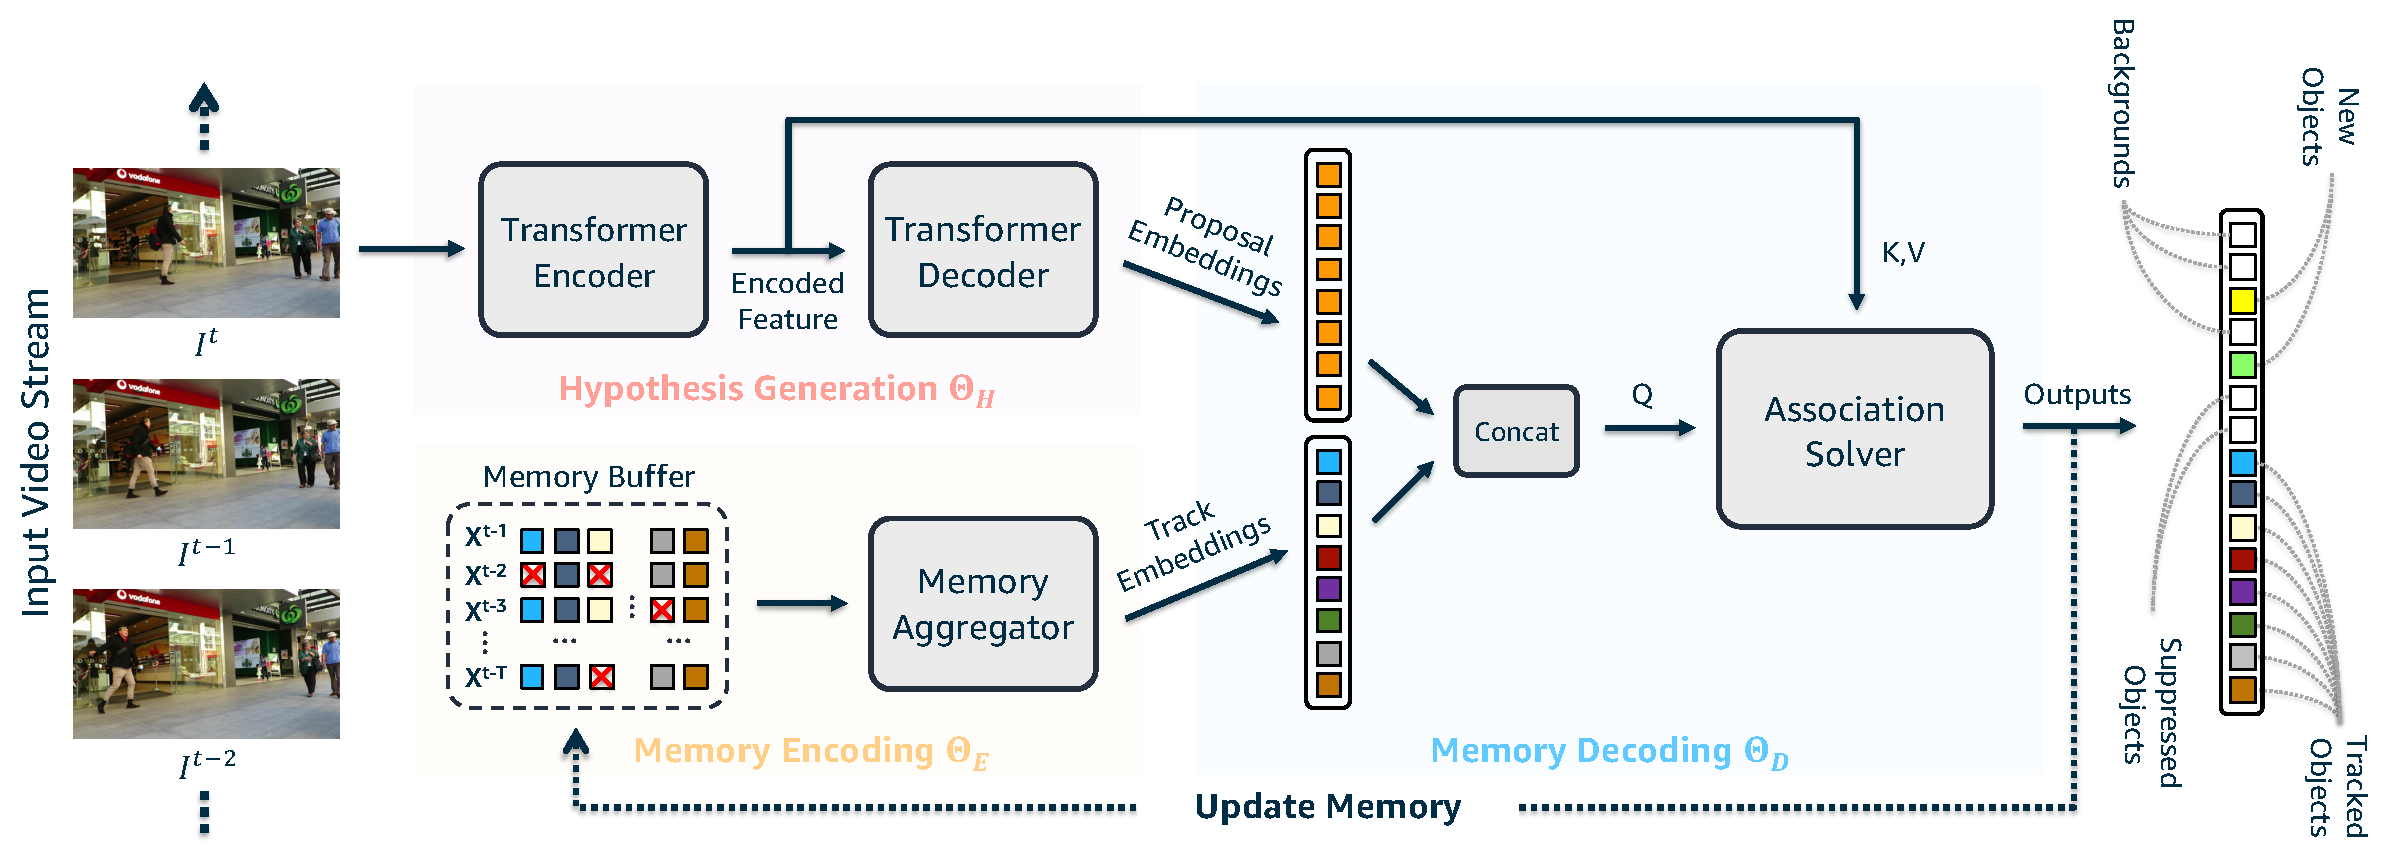
\includegraphics[width=0.97\textwidth]{figures/network.pdf}
    \vspace{-3.5mm}
    \caption{
        \textbf{Visualization of MeMOT}, which runs three main components: 1) a hypothesis generation module $\Theta_H$ that produces object proposals for the current video frame, 2) a memory encoding module $\Theta_E$ that retrieves core information for each tracked objects, and 3) a memory decoding module $\Theta_D$ that solves the object detection and data association tasks simultaneously.
        MeMOT maintains a memory buffer to store long-range states of tracked objects, together with an efficient encoding-decoding process that retrieves useful information for linking objects after a long time span.
        Each hypothetical object is predicted as a new object, a tracked object, or a background region.
    }
    \label{fig:network}
\end{figure*}

\noindent \textbf{Classical Tracking Methods}.
Tracking is well studied in computer vision~\cite{isard1998condensation,babenko2010robust,wu2013online,kristan2015visual}.
Coping with the underlying uncertainties of the tracking results~\cite{isard1998condensation} and object appearances/positions/shapes~\cite{babenko2010robust} has been a central challenge.
Classical non-deep learning methods~\cite{wu2013online} have laid out solid mathematical and statistical foundations.
Specifically, Kalman~\cite{welch1995introduction} and particle filters ~\cite{gustafsson2002particle} are widely adopted for tackling tracking problems~\cite{shen2003probabilistic,hue2001particle,xing2009multi}. The progressive observation-based Bayesian inference method~\cite{xing2010multiple} is proposed for MOT in online sports videos. A spatial and temporal shape representation-based Bayesian framework~\cite{giebel2004bayesian} is proposed for multi-cue 3D deformable object tracking. In these methods,
an optimal filter maintains tracking states that summarize history information and estimate new frame's tracking results. In a linear-Gaussian case, the optimal state can indeed be estimated, while for more general non-linear, non-Gaussian cases, it is difficult to estimate the optimal state with a finite-dimensional state representation. For instance, occlusion in visual multiple object tracking is clearly non-linear and non-Gaussian.
To tackle this challenge, tracking methods~\cite{choi2010multiple,perera2006multi} that can access multiple frames states (offline tracking) is desired.

\vspace{2pt} \noindent \textbf{MOT with CNNs}.
A typical scheme for MOT~\cite{wojke2017simple,feng2019multi,wang2019exploit,chu2019famnet} is ``tracking-by-detection'', which directly uses ready-made detectors~\cite{felzenszwalb2009object,ren2015faster,liu2016ssd,zhou2019objects,ge2021yolox} and focuses on the data association.
% Recent approaches build object detection and data association in the same network.
Tracktor++~\cite{bergmann2019tracking} propagates the bounding boxes of tracked objects as region proposals to the next frame.
CenterTrack~\cite{zhou2020tracking} takes an additional point-based heatmap as input and matches objects anywhere within the receptive field.
JDE~\cite{xu2018joint,wang2019towards,zhang2020fair,li2021semi} is built with two homogeneous branches for object detection and ReID feature extraction, respectively.
Joint detection and tracking models improve the runtime, but sacrifice the tracking recovery after occlusion and cannot reconnect long-term missing objects.

\vspace{2pt} \noindent \textbf{MOT with Transformers}.
Vision Transformers have been successfully applied in image recognition~\cite{carion2020end,dosovitskiy2020image,zhu2020deformable,liu2021swin} and video analysis~\cite{arnab2021vivit,bertasius2021space,sharir2021image,liu2021video} lately.
In tracking, TrackFormer~\cite{meinhardt2021trackformer} and MOTR~\cite{zeng2021motr} simultaneously perform the object detection and association by concatenating the object and autoregressive
track queries as inputs to the Transformer decoder in the next time step.
On the other hand, TransCenter~\cite{xu2021transcenter} and TransTrack~\cite{sun2020transtrack} only use Transformers as feature extractor and recurrently pass track features to aggressively learn aggregated embedding of each object.
TransMOT~\cite{chu2021transmot} still uses CNNs as detector and feature extractor, and learns an affinity matrix with Transformers.
The above work explores the mechanism of representing object states as dynamic embeddings. However, the modeling of long-term spatio-temporal observations and adaptive feature aggregation methods are underdeveloped.

\vspace{3pt} \noindent \textbf{Memory Networks}.
Pioneering work using memory networks has been proposed in NLP~\cite{graves2014neural,weston2014memory,sukhbaatar2015end} by focusing on temporal reasoning tasks such as question answering~\cite{xiong2016dynamic,kumar2016ask} and dialogue systems~\cite{wu2019global}.
Video analysis tasks, such as action recognition~\cite{wu2019long,xu2021long}, and video object segmentation~\cite{oh2019video,lu2020video}, leverage an external memory to store and access time-indexed features in prolonged sequences, significantly improving the ability to remember the past.
Recently, memory networks have been introduced into tracking.
MemTrack~\cite{yang2018learning} reads a residual template from memory and combines it with the initial template to update the representations of targets.
STMTrack~\cite{fu2021stmtrack} guides the information retrieval with the current frame and adaptively obtains all useful information as it needs.
However, these work focuses on single object tracking (SOT), and does not need to concern about the inter-object association.
We propose to use a large spatio-temporal memory to achieve robust object association across time for MOT.


\begin{algorithm}[!t]
    \caption{Key operations of the N-ary sum tree.}
    \label{alg:n_nary_sum_tree_func}
    \begin{algorithmic}[1]
      \Function{updateValue}{idx, value}
          \State node\_idx = \Call{convertToNodeIdx}{idx};
          \State $\Delta$ = value - \Call{getValue}{node\_idx};
          \While{!\Call{isRoot}{node\_idx}}
              \State new\_value = \Call{getValue}{node\_idx} + $\Delta$;
              \State \Call{SetValue}{node\_idx, new\_value};
              \State node\_idx = \Call{getParent}{node\_idx};
          \EndWhile
      \EndFunction
      \\
      \Function{getPrefixSumIdx}{prefixSum}
          \State node\_idx = \Call{getRoot}{\null};
          \While{!isLeaf(node\_idx)}
              \State node\_idx = \Call{getLeftChild}{node\_idx};
              \State partialSum = 0;
              \For{$i$ = 0; $i$ $<$ fan\_out; $i++$}
                  \State sum = partialSum + \Call{getValue}{node\_idx};
                  \If{sum $\geq$ prefixSum}
                      \State break;
                  \EndIf
                  \State partialSum = sum;
                  \State node\_idx = \Call{getNextSibling}{node\_idx};
              \EndFor
              \State prefixSum = prefixSum - partialSum;
          \EndWhile
          \State idx = \Call{convertToDataIdx}{node\_idx};
          \State \Return idx;
      \EndFunction
    \end{algorithmic}
\end{algorithm}

\section{Parallel Prioritized Replay Buffer}\label{sec:parallel_per}
In this section, we discuss in detail the design of our Prioritized Replay Buffer that supports parallel actors and learners. We start by introducing the key operations that need to be supported.
\subsection{Operations}\label{sec:parallel_per_ops}
\subsubsection{Insertion}
Given a new data item $x$, find the next available index $i$ and insert $x$ at $i$. If the Replay Buffer is full, find the index using the eviction policy. Set the priority at index $i$ to $P(i)=P_{\max}$, where $P(i)$ is the priority at index $i$ and $P_{\max}$ is the maximum priority in the Replay Buffer. The most common eviction policy used in existing implementations is First-in-first-out (FIFO).
\subsubsection{Sampling}
Sample a data item $x_i$ according to the probability distribution $Pr(i)=\nicefrac{P(i)}{\sum_{i}P(i)}, i=1,2,\ldots, N$, where $N$ is the size of the Replay Buffer. To do so, we first sample $x$ from uniform distribution $U(0,1)$. Then, we compute the cumulative density function (cdf) as $cdf(i)=\sum_{j=1}^{i}Pr(j), i=1,2,\ldots, N$. Finally, the sampled index $i=cdf^{-1}(x)$. Mathematically, this is equivalent to finding the minimum index $i$, such that the \textbf{prefix sum} of the probability from 0 to $i$ is greater than or equal to $x$:
\begin{align}
    \min_{i}\sum_{j=1}^{i}Pr(i)\geq x \Rightarrow \min_{i}\sum_{j=1}^{i}P(i)\geq x\cdot \sum_{j=1}^{N}P(j)
    \label{eq:prefix_sum}
\end{align}
\subsubsection{Priority retrieval}
Return the priority at index $i$.
\subsubsection{Priority update}
Update the priority at index $i$.

\subsection{Frequency of the Operations and Runtime Requirements} 
As shown in Algorithm~\ref{alg:off_policy_rl}, the insertion is executed once per iteration. The sampling, priority retrieval and priority update are executed once every update\_interval. Directly storing the priority in an array incurs a runtime complexity of $\Theta(N)$ for sampling and $\Theta(1)$ for priority retrieval and priority update. Directly storing the prefix sum in an array incurs a runtime of $\Theta(\log N)$ in sampling, $\Theta(1)$ in priority retrieval and $\Theta(N)$ in priority update. Based on the frequency of the operations, both these implementations incur a overall runtime complexity of $\Theta(N)$. In this paper, we proposed to use $K$-ary sum tree to implement the Prioritized Replay Buffer to achieve $\Theta(\log N)$ runtime complexity for both sampling and priority update and thus for the entire implementation.

\subsection{$K$-ary Sum Tree}\label{sec:sum_tree}
We show an example of a $K$-ary sum tree for $K=4$ in Figure~\ref{fig:sum_tree}. Each node has $K$ child nodes. The value stored in the parent node is the sum of all the values stored in the child nodes. The leaf nodes hold the actual priorities. 

\begin{figure}
    \centering
    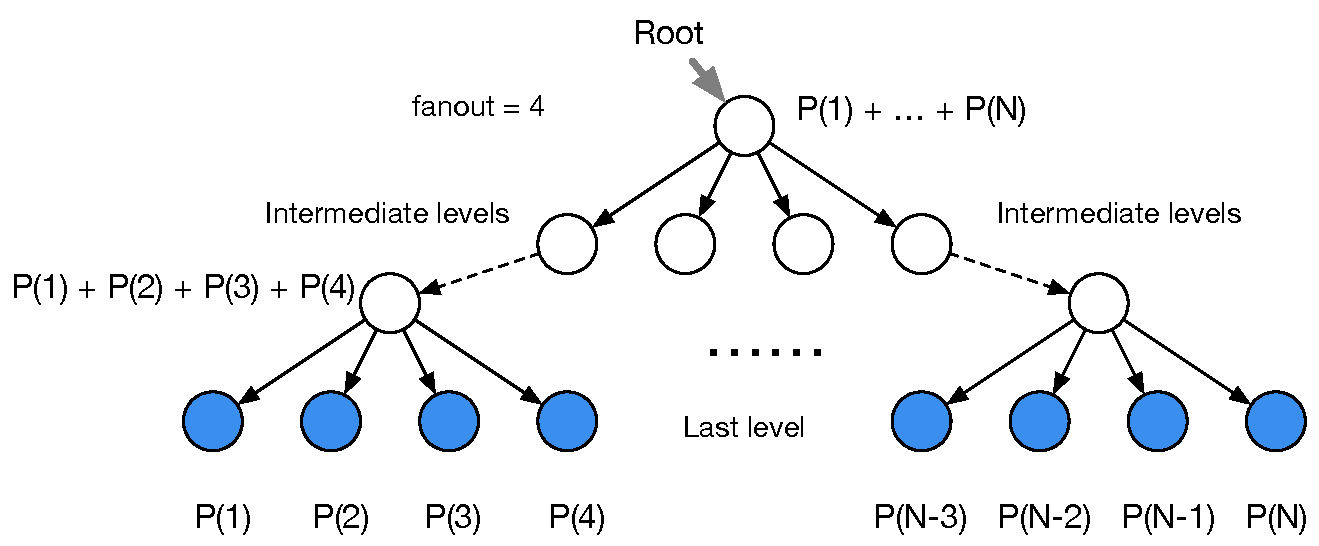
\includegraphics[width=\linewidth]{sum_tree.pdf}
    \caption{The overall structure of a 4-ary sum tree.}
    \label{fig:sum_tree}
\end{figure}

\begin{figure}
    \centering
    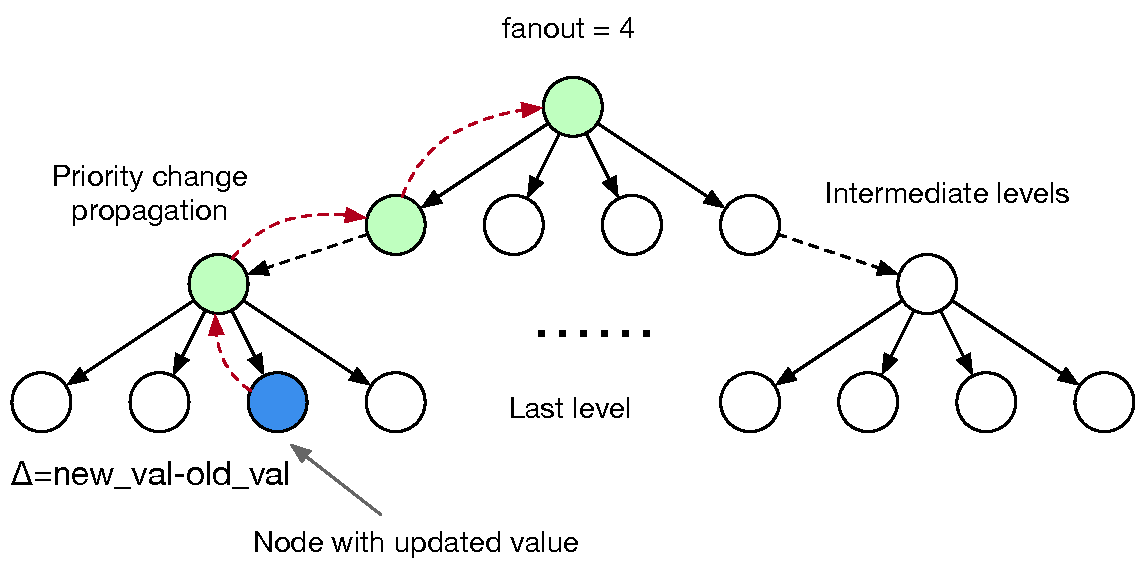
\includegraphics[width=\linewidth]{update_value.pdf}
    \caption{Illustration of the process when updating the value in the $K$-ary sum tree with fanout=4 as shown in Algorithm~\ref{alg:n_nary_sum_tree_func}. The blue node denotes the leaf node that holds the priority. The green nodes denote the intermediate sums that are updated by propagating the change of the priority from the leaf to the root. The red dotted arrow shows the direction of the value propagation.}
    \label{fig:update_value}
\end{figure}

\begin{figure*}
    \centering
    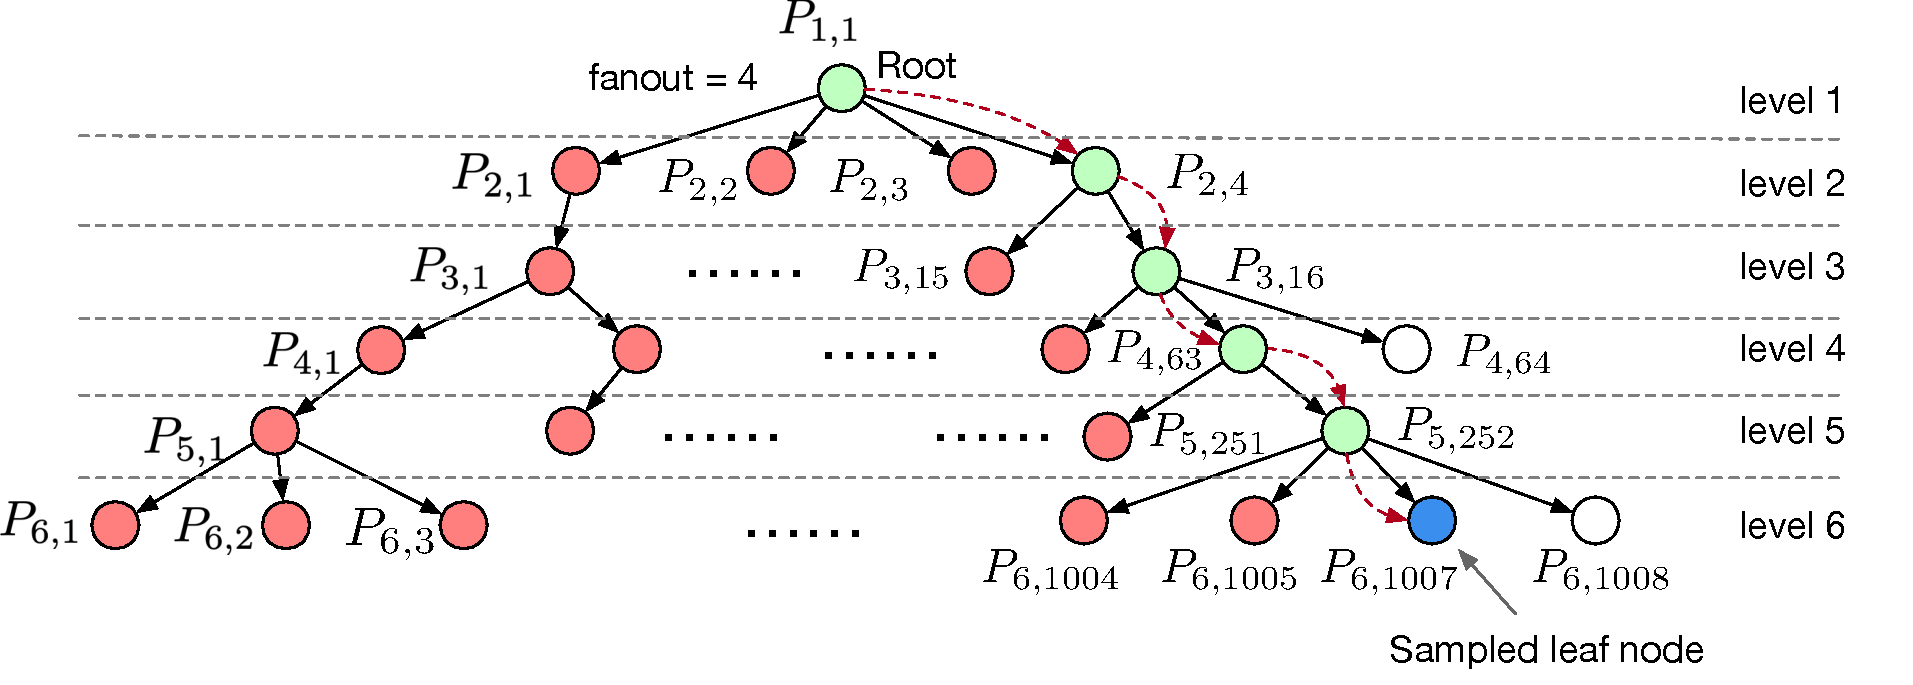
\includegraphics[width=\linewidth]{get_prefix_sum.pdf}
    \caption{Illustration of the process when sampling index according to the priority in the $K$-ary sum tree with fanout=4 as shown in Algorithm~\ref{alg:n_nary_sum_tree_func}. Starting from the root node, the green nodes denote the cutoff node during traversal and the blue node denotes the leaf node sampled. The red dotted arrow shows the direction of the tree traversal.}
    \label{fig:get_prefix_sum}
\end{figure*}

\subsubsection{Priority retrieval}
In order to obtain the priority for the index $i$, we create an array of pointers, each pointing to its corresponding leaf node that holds the priority value. Thus, priority retrieval using $K$-ary sum tree requires $\Theta(1)$ time.

\subsubsection{Priority update}
To update the priority of index $i$, we first obtain the leaf node holding the priority. We compute the change of the priority by subtracting the old value from the new value. Then, we propagate the change of the priority from the leaf node to the root node by traversing along the parent nodes. We show a detailed function in Algorithm~\ref{alg:n_nary_sum_tree_func} and an example in Figure~\ref{fig:update_value}. It is easy to see that this operation requires $\Theta(\log_K N)$ time.

\subsubsection{Prefix sum index computation}
Given a randomly sampled number $x\sim U(0,1)$, the objective is to compute index $i=\min_{i}\sum_{j=1}^{i}P(i)\geq x\cdot \sum_{j=1}^{N}P(j)$ as discussed in Section~\ref{sec:parallel_per_ops}. The sum of all the priorities in the Replay Buffer $\sum_{j=1}^{N}P(j)$ can be computed in $\Theta(1)$ by simply retrieving the value stored in the root node. To design an algorithm that obtains the target index, we start by proving Lemma~\ref{lemma:index_existence} and theorem~\ref{the:sum_tree_prefix}:

\begin{lemma}
    \label{lemma:index_existence}
    Let the value of the $i$-$th$ node at level $m$ be $P_{i,m}$. Assume the height of the tree is $H$. Then, at level $1\leq m\leq H$, there exists index $j$, $1 \leq j \leq K^{m-1}$, such that $\sum_{i=1}^{j}P_{m, i}\geq x\cdot \sum_{i=1}^{N}P(i)$, for any $x\in (0, 1)$.
\end{lemma}
\begin{proof}
    According to the definition, the leaf node holds the priority value. Thus, $P_{i, H}=P(i), \forall i=1,2,\ldots, K^{H-1}$. Since $x\in (0, 1)$, we obtain $x\cdot \sum_{i=1}^{N}P(i)\leq \sum_{i=1}^{N}P(i) \leq \sum_{i=1}^{K^{H-1}}P_{i,H}$. Because the priority values are non-negative, there must exist index $j$, $1 \leq j \leq K^{H-1}$, such that $\sum_{i=1}^{j}P_{H, i}\geq x\cdot \sum_{i=1}^{N}P(i)$. According to the property of the sum tree, the value of the parent is the sum of all its children. Thus, $\sum_{i=1}^{K^{H-1}}P_{H, i}=\sum_{i=1}^{K^{m-1}}P_{m, i}, \forall m=1, 2, \cdots, H-1$. Therefore, the same argument holds for each level. This concludes the proof for Lemma~\ref{lemma:index_existence}.
\end{proof}
\begin{theorem}
    \label{the:sum_tree_prefix}
    Let $j_m=\min_{j'} \sum_{i=1}^{j'}P_{m, i}\geq x\cdot \sum_{i=1}^{N}P(i)$. Then, $j_m$ is the parent node of $j_{m+1}$, $\forall m=1,2,\cdots H-1$.
\end{theorem}
\begin{proof}
    The child nodes of index $j$ at level $m$ are $K\cdot(j-1)+1,\cdots, K\cdot j$ at level $m+1$. According to the definition of the sum tree and the property of $j_m$, we obtain $\sum_{i=1}^{j_m-1}P_{m,i}=\sum_{i=1}^{K\cdot(j_m-1)}P_{m+1, i}< x\cdot \sum_{i=1}^{N}P(i)$. Thus, the index of the cutoff node at level $m+1$ must be $j_{m+1}\geq K\cdot(j_m-1)+1$. Noticing that $\sum_{i=1}^{j_m}P_{m,i}=\sum_{i=1}^{K\cdot(j_m)}P_{m+1, i}\geq x\cdot \sum_{i=1}^{N}P(i)$. Thus, the index of the cutoff node at level $m+1$ satisfies $j_{m+1}\leq K\cdot j_m$. Combining $K\cdot(j_m-1)\leq j_{m+1}\leq K\cdot j_m$, we obtain $j_m$ is the parent node of $j_{m+1}$.
\end{proof}
We refer such node $j_m$ as the \textit{cutoff node} at level $m$. The goal of sampling is to find the index of the cutoff node at the last level of the tree. 
According to Theorem~\ref{the:sum_tree_prefix}, the cutoff node at level $m$ is the parent of the cutoff node at level $m+1$. 
Therefore, we can start from the root node and perform the search only using the child nodes. To obtain which child node is the cutoff node, we maintain a cumulative sum of all the nodes left to the cutoff at each level. Please refer to Algorithm~\ref{alg:n_nary_sum_tree_func} for details.
We also illustrate an example of the process in Figure~\ref{fig:get_prefix_sum}, where $K=4$ and $H=6$.

\subsubsection{Data layout}
Maintaining the explicit tree data structure using pointers significantly degrades the cache performance of modern CPUs. In this work, we implement the tree data structure implicitly using an array as shown in Figure~\ref{fig:data_layout}. The sampling process requires traversing all the nodes under the same parent. To maximize the cache performance, it is desired that each group of child nodes under the same parent is cache aligned. Assume that one cacheline can store $C$ nodes, then we choose $K$, such that $K\%C=0$. We pad the root node with $K-1$ so that it is also cache aligned.

\begin{figure}
    \centering
    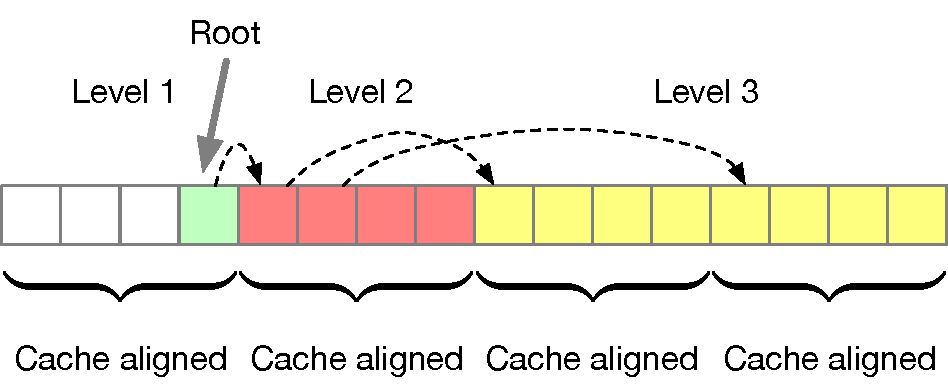
\includegraphics[width=\linewidth]{data_layout.pdf}
    \caption{Data layout of the proposed sum tree with $K=4$. The black arrow shows the first child of the parent node. The color indicates the level of the node in the tree.}
    \label{fig:data_layout}
\end{figure}

\subsubsection{Theoretical performance analysis}
\paragraph{Space complexity}
The space complexity is proportional to the number of nodes in the tree. Assume the size of the Replay Buffer is $N$, which is equal to the number of nodes in the last level of the tree. Thus, the total number of nodes in the tree is: $\Theta(\frac{K^H-1}{K-1})=\Theta(\frac{K^{H-1}\cdot K-1}{K-1})=\Theta(\frac{N\cdot K-1}{K-1})=\Theta(N+\frac{N-1}{K-1})$. Clearly, as $K$ increases, the space complexity reduces due to the decrease of the number of intermediate nodes.

\paragraph{Runtime complexity}
It is clear that the priority retrieval runs in $\Theta(1)$ and priority update runs in $\Theta(\log_K N)$. For prefix sum index computation, the loops runs $H=\ceil{\log_K N} + 1$ times. The memory access inside loop has $\nicefrac{K}{C}$ cache misses and $K\cdot(1-\nicefrac{1}{C})$ cache hit, where $C$ is the number of nodes in one cacheline. Thus, the time complexity of prefix sum index computation is $\Theta((\log_K N+1)(T_{miss}\cdot\frac{K}{C}+T_{hit}\cdot K\cdot(1-\nicefrac{1}{C})))$, where $T_{miss}$ is the execution time of one cache miss and $T_{hit}$ is the execution time of one cache hit. Note that this function has a local minimum in terms of $K$. In practice, we profile the performance of various $K$ values based on the size of the cacheline and choose the one that yields the best performance.

\subsection{Thread-safe Prioritized Replay Buffer}\label{sec:thread_safe_prb}
In order to support parallel actors and learners, it is crucial to design thread-safe prioritized Replay Buffer. We summarize the resource utilization of various operations in Table~\ref{table:resource_util}. We design the thread-safe prioritized replay buffer using locking mechanism such that the duration of holding a lock is minimized. 

\subsubsection{Synchronization of the sum tree}
We use two locks to synchronize the sum tree: one to synchronize the read/write of the last level of the tree and the other to synchronize the read/write of all the levels. A detailed procedure of priority update and priority retrieval is shown in Algorithm~\ref{alg:sync_replay_buffer}. Using this technique, reading of the priority value and updating of the intermediate levels of the sum tree can be executed in parallel. Note that it will cause inconsistencies if we acquire the global\_tree\_lock after releasing the last\_level\_lock lock when two priority update queries arrive at the same time.

\subsubsection{Synchronization of insertion and sampling}
During insertion, the Replay Buffer finds an available index. Then, it writes the data to the storage and updates the priority to the maximum priority in the Replay Buffer. Compared with index searching and priority update, data writing takes more time due to explicit copy of the memory data. Thus, it is important not to hold the lock while performing the data writing. To do so, we propose \textit{lazy writing}: 1) We set the priority to zero atomically; ii) we perform data writing; iii) we reset the priority to the maximum priority in the Replay Buffer atomically. Since the priority is zero during data writing, it will never be sampled. This makes sampling only needs to synchronize prefix sum index computation. A detailed procedure is shown in Algorithm~\ref{alg:sync_replay_buffer}.


\begin{algorithm}[!t]
    \caption{Synchronization of the Prioritized Replay Buffer}
    \label{alg:sync_replay_buffer}
    \begin{algorithmic}[1]
        \Function{PriorityUpdate}{idx, new\_priority}
            \State \Call{Acquire}{global\_tree\_lock};
            \State \Call{Acquire}{last\_level\_lock};
            \State \Call{UpdateLastLevel}{\null};
            \State \Call{Release}{last\_level\_lock};
            \State \Call{UpdateIntermediateLevel}{\null};
            \State \Call{Release}{global\_tree\_lock};
        \EndFunction
        \\
        \Function{PriorityRetrieval}{idx}
            \State \Call{Acquire}{last\_level\_lock};
            \State priority = \Call{getPriority}{idx};
            \State \Call{Release}{last\_level\_lock};
            \State \Return priority;
        \EndFunction
        \\
        \Function{Insert}{idx, data}
            \State \Call{UpdatePriority}{idx, 0};
            \State \Call{WriteToStorage}{idx, data};
            \State \Call{UpdatePriority}{idx, max\_priority};
        \EndFunction
        \\
        \Function{Sample}{\null}
            \State \Call{Acquire}{global\_tree\_lock};
            \State idx, priority = \Call{getPrefixSumIndex}{\null};
            \State \Call{Release}{global\_tree\_lock};
            \State \Return idx, priority;
        \EndFunction
    \end{algorithmic}
\end{algorithm}


\begin{table}[!t]
    \centering
    \caption{Resource utilization of various operations}
    \vspace{-1em}
    \begin{tabular}{cc}
        \toprule
        Operations & Resource Utilization  \\
        \midrule
        Insertion & modify the entire tree, modify the storage \\
        Sampling & access the entire tree, access the storage \\
        Priority retrieval & access the last level of the tree \\
        Priority update & modify the entire tree \\
        \bottomrule
    \end{tabular}
    \label{table:resource_util}
\end{table}

\subsubsection{Write after read vs. read after write}
The parallelism of the priority update and the data sampling causes data dependency issues: the same data is sampling using the old priority before the new priority gets updated (write after read). Mathematically, only read after write is valid and write after read produces inconsistent results. However, it has little impact in practice as neural network training is stochastic in nature and robust to such transient inconsistencies.


\section{Overall Framework}
\begin{figure*}
    \centering
    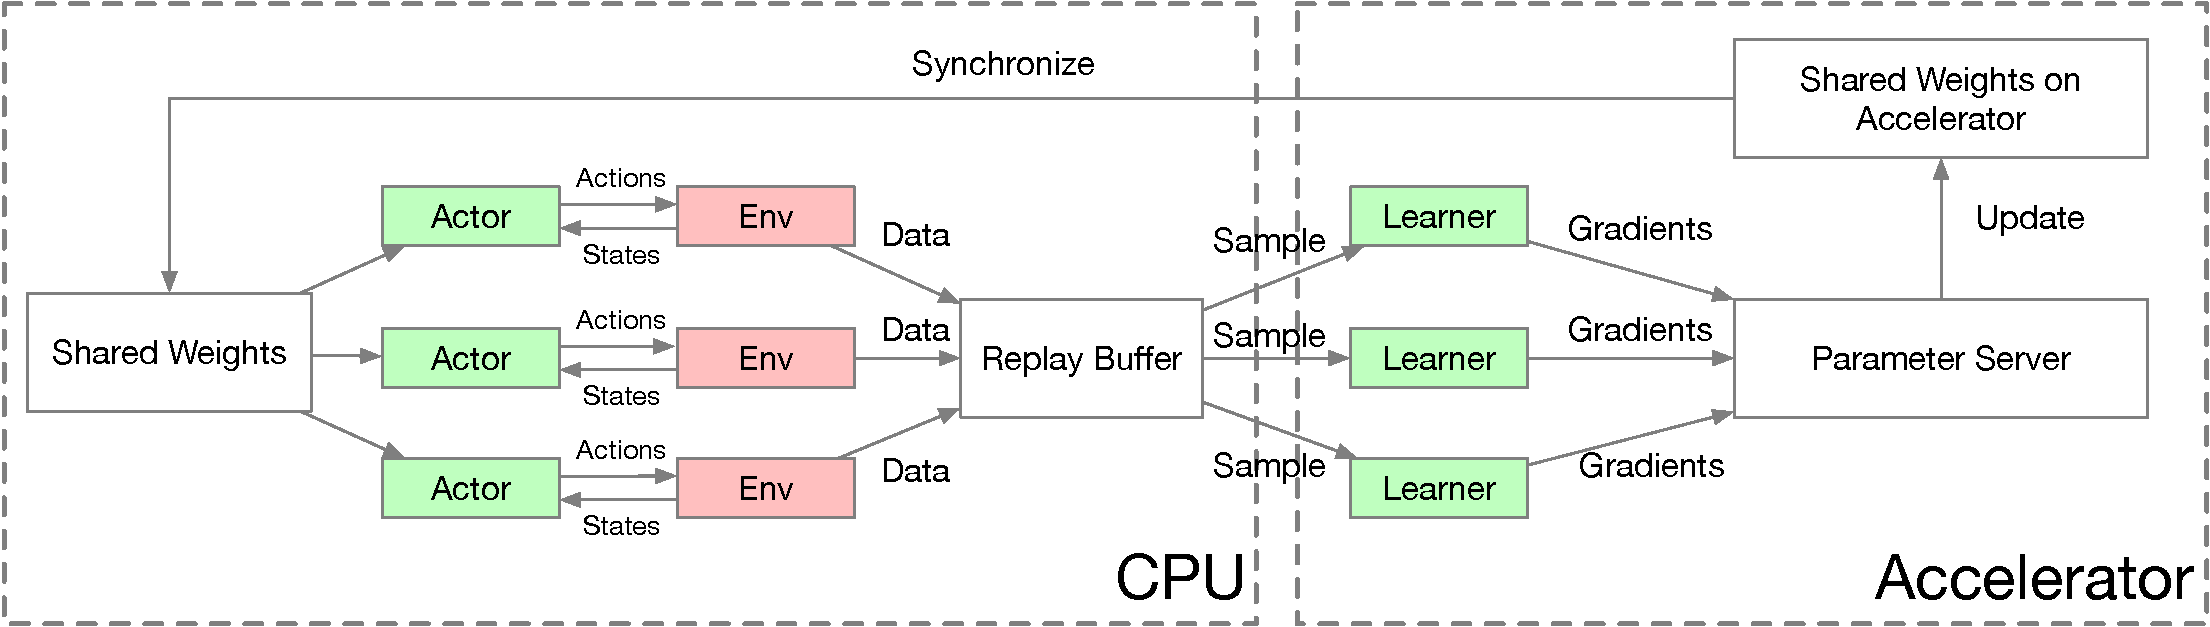
\includegraphics[width=\linewidth]{overall_system.pdf}
    \caption{Overall system architecture}
    \label{fig:overall_system}
\end{figure*}

The overall system architecture is shown in Figure~\ref{fig:overall_system}. We employ parallel actors to collect data and parallel learners to compute the gradients for neural network weights update. 

\subsection{Asynchronous Actors}
Asynchronous actors collect the data simultaneously by interacting with their own instance of the environment using the shared weights. The data is then added to the Replay Buffer. It is worth noting that no synchronization is required because the inference doesn't alter the weights.

\subsection{Parallel Learners}
Deploying parallel actors increases the throughput of data collection. In order to increase the throughput of the learning, we employ parallel learners with a central parameter server \cite{parameter_server}. Each learner independently samples one batch of data from the Replay Buffer and computes the sub-gradients. The parameter server aggregates the gradients and updates the weights.

\subsection{Framework Specification}
Our framework supports a wide range of reinforcement learning algorithms including DQN \cite{dqn}, DDQN \cite{double_q_learning}, DDPG \cite{ddpg}, SAC \cite{sac}, TD3 \cite{td3} and so on. The target platform of our framework is processor + accelerator platforms, where the processor is the CPU the accelerator is either the GPU or the FPGA. The input of our framework includes:
\begin{itemize}
    \item The overall throughput of the data collection vs. the number of CPU cores.
    \item The overall throughput of the data consumption vs. the number of CPU cores.
    \item Total number of cores in the CPU.
\end{itemize}
The throughput of the data collection by a single actor is affected by i) the time of a single environment step function defined in Section~\ref{sec:mdp}; ii) The specifications of the neural networks used in the actors including the architecture (fully-connected vs. convolution networks), the size of each layer, etc. iii) the speed of the processor. The throughput of a single learner is affected by i) the reinforcement learning algorithm; ii) the optimizer iii) the speed of the accelerator.

\subsection{Design Space Exploration}\label{sec:design_space_exp}
The objective of is to choose the number of actor threads and the number of learner threads such that the ratio between the throughput of the data collection vs. data consumption is the same as the single thread implementation (update\_interval denoted in Algorithm~\ref{alg:off_policy_rl}). In order to obtain the allocation of the cores, we profile the overall throughput of the data collection vs. the number of CPU cores and denote the curve as $f_{a}(x)$, where $x$ is the number of cores. Similarly, we profile the overall throughput of the data consumption vs. the number of CPU cores and denote the curve as $f_{l}(x)$. Let the total number of CPU cores be $M$. Then, the design space exploration is the solution of equation~\ref{eq:design_space}:
\begin{align}
    \label{eq:design_space}
    f_{a}(x_a) &= \text{update\_interval}\times f_{l}(x_l) \nonumber\\
    x_a + x_l &\leq M
\end{align}
where $x_a$ and $x_l$ is the allocated number of cores for actors and learners, respectively.
If the parallel actors and/or learners are deployed on an accelerator such as GPU or FPGA, instead of CPU, profiling similar to the one described above can be used to perform the design space exploration. 


In this section, we leverage the \snact\  to empirically validate the techniques introduced in \Cref{sec:techniques}. First, to concretize the capability gap between open-source and closed LLMs, we demonstrate that OpenAI GPT-4 API can have substantially higher success rate than representative open-source LLMs in~\Cref{subsec:cap_gap}. 
We then show in~\Cref{subsec:boost} that the simple techniques in~\Cref{sec:techniques} can boost open-source LLMs to achieve success rates competitive to in-context-learning with GPT-4 APIs\footnote{GPT-4 tuning APIs were not released by the time this work is done.} in four out of the eight tasks.
Through ablation studies in~\Cref{subsec:abl}, we additionally show that model alignment does the heavy lifting for boosting open-source LLMs, while system prompt and in-context learning robustify LLMs for further improvement. 

\subsection{Experiment Setup}
To establish strong baselines, we use GPT-4 API as the representative closed LLM in our study because it attains the leading accuracy in mainstream NLP tasks. 
In our study, we compare LLAMA-30B \cite{touvron2023llama}, StarCoder \cite{li2023starcoder} and CodeGen-16B-mono \cite{nijkamp2022codegen} to GPT-4. LLAMA represents open research models, while StarCoder and CodeGen are publicly available for both research and commercial purposes. We choose these three models due to their superior performance on \snact\  among open-source models as shown in~\Cref{tab:baselines_over_models}\footnote{Surprisingly, we observe that for tool manipulations, open-source LLMs instruction-tuned for conventional NLP tasks do not outperform their base models before tuning.}. 
In our experiments, we consider the zero-shot setting as the out-of-the-box configuration where only API documentation is provided without any demonstration examples. We use this configuration to understand the initial gap in capabilities among models. We then incorporate all available techniques on top of this initial configuration to assess their benefits. 
For the original Tabletop dataset~\cite{liang2022code}, which includes examples in a few-shot setting without explicit API definitions, we only evaluate settings with in-context demonstrations. 
More detailed setup information is included in \Cref{sec:app_exp_details}. We run each job 3 times with different random seeds and report average accuracy. The variation is minimal, so we ignore them in the main paper but report them in appendix.





\subsection{Capability Gap}
\label{subsec:cap_gap}
\Cref{tab:baselines} exhibits significant disparities in tool manipulation between the closed GPT-4 API and open-source models in the out-of-the-box zero-shot setting. 
For simpler tasks, namely Open Weather and the Cat API, which require only one API call for each goal, the open-source models exhibit success rates up to $74\%$ lower than GPT-4. 
Furthermore, on all the remaining tasks other than the Webshop, none of the LLAMA, the StarCoder and the CodeGen model can reach meaningful accuracy or compare with GPT-4. 
These results highlight an opportunity to enhance open-source LLMs.
% for tool manipulation.
% 1. Large gap across tasks
% 2. Some tasks demonstrate zero.
% 3. One interesting observation is that in context.

\begin{table}[]
\caption{Capability gap in tool manipulation is substantial between closed API and open-source LLMs in the out-of-the-box zero-shot setting. Using model alignment, the in-context demonstration retriever and the system prompt, open-soured LLMs attain significant boost in success rate. GPT-4 is enhanced with the retriever and system prompt.
% ; model alignment tuning does not apply to GPT-4 because tuning API is not available when we carry out the experiment.
Tabletop is only evaluated in the few-shot fashion. 
% Average success rate over 3 random seeds are reported. 
}
\label{tab:baselines}
\begin{adjustbox}{max width=\textwidth}

\setlength{\tabcolsep}{4pt}
\begin{tabular}{@{}cccccccccc@{}}
\toprule
                                          & \textbf{Open}                           & \textbf{The Cat}                    & \textbf{Home}        & \textbf{Trip}        & \textbf{Google}      &                                        & \multicolumn{2}{c}{\textbf{WebShop}}        &                                     \\
\multirow{-2}{*}{\textbf{Task}}           & {\color[HTML]{1F1F1F} \textbf{Weather}} & {\color[HTML]{1F1F1F} \textbf{API}} & \textbf{Search}      & \textbf{Booking}     & \textbf{Sheets}      & \multirow{-2}{*}{\textbf{VirtualHome}} & \textbf{Long}        & \textbf{Short}       & \multirow{-2}{*}{\textbf{Tabletop}} \\
\midrule
\textit{\textbf{Zero-shot Baseline}}      & \multicolumn{1}{l}{}                    & \multicolumn{1}{l}{}                & \multicolumn{1}{l}{} & \multicolumn{1}{l}{} & \multicolumn{1}{l}{} & \multicolumn{1}{l}{}                   & \multicolumn{1}{l}{} & \multicolumn{1}{l}{} & \multicolumn{1}{l}{}                \\
GPT-4                                          & 81.3            & 97.4            & 76.6            & 91.5            & 5.7             & 40.8 / 8.0  & \multicolumn{2}{c}{0.0}                    & -                    \\
LLaMA-30b                                     & 39.0            & 49.0            & 0.0             & 0.0            & 0.0             & 78.0 / 0.3  & \multicolumn{2}{c}{0.0}                    & -                    \\
StarCoder                                     & 32.0            & 71.0            & 7.0             & 13.3            & 5.9             & 22.0 / 3.7  & \multicolumn{2}{c}{0.0}                    & -                    \\
CodeGen-16B-mono                              & 7.0           & 78.0            & 0.0             & 0.0            & 1.4             & 4.0/ 1.0  & \multicolumn{2}{c}{0.0}                    & -                    \\

\midrule
\textit{\textbf{Enhanced w/ techniques}}      & \multicolumn{1}{l}{}                    & \multicolumn{1}{l}{}                & \multicolumn{1}{l}{} & \multicolumn{1}{l}{} & \multicolumn{1}{l}{} & \multicolumn{1}{l}{}                   & \multicolumn{1}{l}{} & \multicolumn{1}{l}{} & \multicolumn{1}{l}{}                \\
GPT-4                                      & 99.0                                    & 98.0                                & 98.0                 & 99.2                 & 68.6                 & 29.0 / 21.7                            & 0.0                  & 0.0                  & 83.8                                \\
LLaMA-30b                                     & 100.0           & 94.0            & 87.0            & 85.8            & 2.9             & 16.0 / 24.3 & 0.0             & 0.0             & 7.5             \\
StarCoder                                     & 99.0            & 97.0            & 83.0            & 80.8            & 21.2            & 31.0 / 18.4 & 0.0             & 0.0             & 13.9            \\
CodeGen-16B-mono                              & 97.7            & 99.0            & 82.0            & 77.5            & 19.8            & 29.0 / 17.2 & 0.0             & 3.5             & 16.2                    \\
\bottomrule
\end{tabular}
\end{adjustbox}
% \vspace{-1em}
\end{table}


% \begin{table}[]
% \caption{Capability gap in tool manipulation is substantial between closed API and open-source LLMs in the out-of-the-box zero-shot setting. Using model alignment, the in-context demonstration retriever and the system prompt, open-soured LLMs attain significant boost in success rate. GPT-4 is enhanced with the retriever and system prompt.
% % ; model alignment tuning does not apply to GPT-4 because tuning API is not available when we carry out the experiment.
% Tabletop is only evaluated in the few-shot fashion.
% }
% \label{tab:baselines}
% \begin{adjustbox}{max width=\textwidth}

% \setlength{\tabcolsep}{4pt}
% \begin{tabular}{@{}cccccccccc@{}}
% \toprule
%                                           & \textbf{Open}                           & \textbf{The Cat}                    & \textbf{Home}        & \textbf{Trip}        & \textbf{Google}      &                                        & \multicolumn{2}{c}{\textbf{WebShop}}        &                                     \\
% \multirow{-2}{*}{\textbf{Task}}           & {\color[HTML]{1F1F1F} \textbf{Weather}} & {\color[HTML]{1F1F1F} \textbf{API}} & \textbf{Search}      & \textbf{Booking}     & \textbf{Sheets}      & \multirow{-2}{*}{\textbf{VirtualHome}} & \textbf{Long}        & \textbf{Short}       & \multirow{-2}{*}{\textbf{Tabletop}} \\
% \midrule
% \textit{\textbf{Zero-shot Baseline}}      & \multicolumn{1}{l}{}                    & \multicolumn{1}{l}{}                & \multicolumn{1}{l}{} & \multicolumn{1}{l}{} & \multicolumn{1}{l}{} & \multicolumn{1}{l}{}                   & \multicolumn{1}{l}{} & \multicolumn{1}{l}{} & \multicolumn{1}{l}{}                \\
% GPT-4                                      & 70.0                                    & 80.0                                & 70.0                 & 45.0                 & 5.7                  & 29.0 / 9.5                             & \multicolumn{2}{c}{0.0}                     & -                                   \\
% LLaMA-30b                                 & 6.0                                     & 5.0                                 & 0.0                  & 0.0                  & 0.0                  & 3.0 / 0.1                              & \multicolumn{2}{c}{0.0}                     & -                                   \\
% LLaMA-30b                                 & 6.0                                     & 5.0                                 & 0.0                  & 0.0                  & 0.0                  & 3.0 / 0.1                              & \multicolumn{2}{c}{0.0}                     & -                                   \\
% CodeGen-16B-mono                          & 12.0                                    & 47.0                                & 0.0                  & 0.0                  & 0.0                  & 0.0 / 0.6                              & \multicolumn{2}{c}{0.0}                    & -                                   \\
% \midrule
% \textit{\textbf{Enhanced w/ techniques}}      & \multicolumn{1}{l}{}                    & \multicolumn{1}{l}{}                & \multicolumn{1}{l}{} & \multicolumn{1}{l}{} & \multicolumn{1}{l}{} & \multicolumn{1}{l}{}                   & \multicolumn{1}{l}{} & \multicolumn{1}{l}{} & \multicolumn{1}{l}{}                \\
% GPT-4                                      & 99.0                                    & 98.0                                & 98.0                 & 99.2                 & 68.6                 & 29.0 / 21.7                            & 0.0                  & 0.0                  & 83.8                                \\
% GPT-4                                      & 99.0                                    & 98.0                                & 98.0                 & 99.2                 & 68.6                 & 29.0 / 21.7                            & 0.0                  & 0.0                  & 83.8                                \\
% LLaMA-30b & 100.0 & 95.0 & 86.0 & 85.8 & 2.9 & 15.0 / 26.4 & 0.0 & 0.0 & 7.6 \\
% CodeGen-16B-mono                          & 99.0                                    & 99.0                                & 83.0                 & 76.7                 & 18.6                 & 37.0 / 19.3                            & 0.0                  & 13.2                 & 16.2                               \\
% \bottomrule
% \end{tabular}
% \end{adjustbox}
% % \vspace{-1em}
% \end{table}
\subsection{Boosting open-source LLMs}
\label{subsec:boost}
To boost the open-source LLMs, we first perform model alignment using programmatially generated data. We then apply a system prompt and a 3-shot demonstration retriever during inference. Given GPT-4 does not provide tuning APIs, we enhance the out-of-the-box GPT-4 with the same system prompt and demonstration retriever as the baseline. The improvements from the combined enhancement techniques are shown in~\Cref{tab:baselines}, where the success rates of the open-source LLMs can improve up to $90\%$. As a result, the open-source models achieve competitive or better success rates on 4 out of 8 tasks, including Open Weather, the Cat API, VirturalHome and WebShop. Moreover, on Home Search and Trip Booking, the gap between the LLAMA model and the GPT-4 API is reduced to $11\%$ and $13.4\%$ respectively, compared to the initial gap of up to $91\%$. Despite the fact that open-source models are still lagging behind on the Google Sheets and Tabletop, these observations show that \emph{our recipe can significantly improve the performance of open-source LLMs and attain success rates comparable to GPT-4 API on many of the \snact\  tasks}.

\paragraph{Human supervision} To identify the practicality of an enhancement recipe, the amount of required human supervision is a crucial factor. In our approach, human supervision is primarily in the form of in-context demonstration examples and alignment data templates.
Regarding the demonstration examples, we provide $10$ to $83$ examples for each task as shown in~\Cref{tab:all_tasks}, except for WebShop given its difficulty in advanced reasoning.
% and the ones in VirtualHome, Webshop and Tabletop are already provided in their original datasets.
As shown in~\Cref{tab:training_data}, the number of templates for alignment data is typically less than $100$ for each task. We observe that providing these supervisions takes one developer day on average, making it practical in terms of the time cost on human supervision.
% \comment{QT: need the statistics on volume of templates for each task and maybe also total generated alignment example count}


\paragraph{Remaining challenges} In our experiments, we observe that the boosted open-source LLMs still have relatively low success rates on tasks that require advanced reasoning, such as Google Sheets, WebShop and Tabletop tasks. This implies the need to further enhance the reasoning capabilities of open-source models. We are excited about the prospect of more exploration from the community to address the challenges for tool manipulation on these complex tasks.



% % 1. Compared 3 trick open sourced to GPT + 2 things for GPT
% 2. Discuss a few examples
% 3. Supervision needed
% 4. Remaining challenges

\subsection{Ablation Study}
\label{subsec:abl}

\begin{wraptable}[14]{r}{6cm}
\vspace{-12pt}
\caption{The number of \snact~tasks improved (+N) or hurt (-N) over the baselines when adding or dropping techniques.}
\label{tab:breakdown}
\begin{adjustbox}{max width=\linewidth}
\setlength{\tabcolsep}{2pt}
\begin{tabular}{@{}lccc@{}}
\toprule
               & LLaMA & StarCoder & CodeGen \\
\midrule
\textbf{Zero-shot} & - & - & -                                                \\
+ Sys. Prompt       & +4 & +4 & +4                                               \\
+ 3-shot & +8 & +8 & +8                                                \\
+ Alignment   & +7 & +7 &+7                                     \\  
\midrule
\textbf{Full system} & - & - & -                                                \\
- Sys. Prompt       & -0 & -2 & -3                                                \\
- 3-shot    & -3 & -4 & -5                                                 \\
- Alignment  & -5 & -5 & -7                                      \\        
\bottomrule
\end{tabular}
\end{adjustbox}
\end{wraptable} 
% To break down the contribution of model alignment, in-context demonstration and sysmtem prompts, we ablate these techniques in two ways in~\Cref{tab:breakdown}. We first apply one technique a time on top of the out-of-the-box zero-shot configuration and show the impacts in isolation. We then take the combination of the techniques and remove one at a time to evaluate the relative contributions in the context of the full system.
% The full results of the experiments in this section can be found in \Cref{tab:baselines_over_techniques}.

% \paragraph{Impact of techniques} 
% As seen in~\Cref{tab:breakdown}, both 3-shot in-context demonstration and model alignment can bump up the success rate of all the tasks, while system prompts only boosts simple tasks requiring relatively fewer number of API call for each goal.

% \paragraph{System ablation} In the context of full system with all three techniques, we can observe that solely removing model alignment triggers success rate degradation in up to 7 tasks in~\Cref{tab:breakdown}, while removing either in-context demonstration or system prompt hurts up to 5 tasks. We notice that the tasks that are not significantly hurt when removing techniques are the ones that have relatively low success rate (usually <20\%) even in the full system. Thus those accuracy changes are subject to high variance and fluctuation.


% To break down the contribution of model alignment, in-context demonstration and sysmtem prompts, we ablate these techniques in two ways. 
We break down the contribution of the techniques in two ways.
First, we apply each technique individually on top of the out-of-the-box zero-shot configuration and evaluate its impact. 
As shown in~\Cref{tab:breakdown}, both the 3-shot in-context demonstration and model alignment techniques bump up the success rates across all tasks, while the system prompt only benefits simple tasks that involve relatively fewer API calls for each goal.

Next, we consider the combination of all techniques and remove them one at a time to evaluate their relative contributions within the full system. As shown in in~\Cref{tab:breakdown}, solely removing model alignment triggers success rate degradation in up to 7 tasks, while removing either in-context demonstration up to 5 tasks and dropping system prompt up to 3. We notice that the tasks that are not significantly impacted when removing techniques are typically the ones with relatively low success rate (usually <20\% even in the full system). Thus, those accuracy changes are hypothetically subject to high variance and fluctuation.
The full results from the experiments in this section can be found in \Cref{tab:baselines_over_techniques}.



% \textbf{Greatly reduce the gap between open- and close-source models}. There is a great gap between open-source models and closed models out-of-the-box in the zero-shot setting. However, when armed with the techniques we provided, the open-source model are dramatically improved from almost non-usable (e.g. the accuracy of LLaMA is below 10\% for most of the tasks) to GPT-4 level on 6 out of 8 tasks, even though the GPT-4 can also benefit from those techniques. 

% \textbf{Our proposed techniques are effective}. Comparing with the zero-shot baseline, every single technique - system prompting, few-shot learning, alignment tuning - can individually bump up the model performance universally across different tasks. Alignment tuning and in-context learning can each close the gap in 5 out of 8 tasks, while deliminate major gap in the rest, when comparing with the GPT-4 zero-shot baseline.

% \textbf{Minimum human supervision's needed.} Show the amount of human labor needed for curate demonstration examples and tuning templates. 

% \subsection{Techniques Contribution Breakdown}
% \label{subsec:abl}


% To understand the contribution of each task, we compute the average success rate of the first 4 tasks on LLaMA and CodeGen, by incrementally removing techniques from the joint setting. We exclude the last four tasks from \snact~ because of their highly variant results (we didn't fully exploit the tuning) \comment{rephrase me to align with 6.1}. As shown in \Cref{tab:breakdown}, combining the three techniques together delivers the best model performance, indicating the techniques are complimentary to each other. Also, we confirm again that tuning is the most beneficial techniques to bump up the open-source model accuracy.


% Describe limitations and any potential negative societal impacts


In this paper, we answer the question \emph{can we enhance open-source LLMs to compete with leading closed LLM APIs in tool manipulation, with practical amount of human supervision}. 
Drawing from our observations of the common tool manipulation failures and insights from the literature on conventional NLP tasks with LLM, we propose to instantiate model alignment with programmatical data generation, system prompts, and in-context demonstration retrievers to improve the tool manipulation capability of open-source models.
To comprehensively evaluate the impact of these techniques, we create the \textit{\snact}, a benchmark consisting of diverse software tools for real-world tasks. 
Our results demonstrate that these techniques can make the leading open-source LLMs competitive with the OpenAI GPT-4 in $4$ out of $8$ \snact\  tasks, all achieved with a practical amount of human labeling effort.


\bibliographystyle{IEEEtran}
\bibliography{bib/chi_bib}

\end{document}
